\documentclass[a4paper,12pt]{article}
\usepackage[utf8]{inputenc}
\usepackage[german]{babel}
\usepackage{amsmath}
\usepackage{amssymb}
\usepackage{amsthm}
\usepackage{geometry}
\usepackage{graphicx}
\usepackage[hidelinks]{hyperref}
\usepackage{listings}
\usepackage{xcolor}
\usepackage{enumitem}
\usepackage{microtype}
\usepackage{booktabs}
\usepackage{siunitx}
\usepackage{float}

\geometry{margin=2.5cm}

\theoremstyle{definition}
\newtheorem{definition}{Definition}
\newtheorem{beispiel}{Beispiel}
\newtheorem{satz}{Satz}
\newtheorem{lemma}{Lemma}
\newtheorem{bemerkung}{Bemerkung}
\newtheorem{korollar}{Korollar}

\setlist[itemize,1]{label=--}

% ---------- Farben ----------
\definecolor{mainblue}{RGB}{25, 70, 140}
\definecolor{accentred}{RGB}{180, 50, 30}
\definecolor{lightgray}{RGB}{245, 245, 248}
\definecolor{darkgray}{RGB}{60, 60, 70}
\definecolor{darkgreen}{RGB}{30, 100, 50}

\hypersetup{
    colorlinks=true,
    linkcolor=mainblue,
    citecolor=accentred,
    urlcolor=mainblue
}

\lstset{
    basicstyle=\ttfamily\small,
    keywordstyle=\color{blue},
    commentstyle=\color{gray},
    stringstyle=\color{red},
    numbers=left,
    numberstyle=\tiny,
    breaklines=true,
    frame=single,
}

\title{Drehmoment-Drehzahl-Charakteristiken von\\
Elektrischen Traktionsmotoren in Elektrofahrzeugen:\\
Mathematische Grundlagen, Modellierung und\\
Systemanalyse}
\author{Stephan Epp}
\date{25. Juni 2026}

\begin{document}

\maketitle

\begin{abstract}
Diese Arbeit behandelt die mathematischen und physikalischen Grundlagen der
Drehmoment-Drehzahl-Kennlinien permanentmagneterregter Synchronmaschinen (PMSM)
als Traktionsantriebe in Elektrofahrzeugen (EV). Es werden formal der konstante
Drehmomentbereich, der Konstantleistungsbereich (Feldschwächung), die
Leistungsbilanz sowie das regenerative Bremsen hergeleitet und bewiesen.
Anhand eines Referenzmotors mit $T_{\max} = \SI{250}{\newton\metre}$,
$P_{\max} = \SI{104{,}7}{\kilo\watt}$, $n_{\mathrm{base}} = \SI{4000}{RPM}$ und
$n_{\max} = \SI{12000}{RPM}$ werden alle Aussagen quantitativ untermauert und
mittels Matplotlib-Grafiken veranschaulicht. Ein umfangreicher Ausblick
beleuchtet zukünftige Forschungsrichtungen in Motordesign, Regelungstechnik,
Thermomanagement und Fahrzeugsystemintegration.
\end{abstract}

\tableofcontents
\newpage

% ============================================================
\section{Einführung}
% ============================================================

Der elektrische Antriebsstrang moderner Elektrofahrzeuge unterscheidet sich
grundlegend vom Verbrennungsmotor. Während konventionelle Motoren ein eng
begrenztes Drehzahlband mit nutzbarem Drehmoment aufweisen und daher mehrstufige
Getriebe benötigen, deckt der elektrische Traktionsmotor ein breites Drehzahlspektrum
mit hohem Drehmoment ab. Das Herzstück dieser Eigenschaft ist die
\emph{Drehmoment-Drehzahl-Kennlinie} (engl.\ \emph{torque-speed characteristic}),
welche das Betriebsverhalten des Motors über den gesamten Drehzahlbereich beschreibt.

\subsection{Motivation und Bedeutung}

Das Drehmoment-Drehzahl-Profil bestimmt unmittelbar:
\begin{itemize}
    \item die \textbf{Beschleunigungsfähigkeit} (Anfahrmoment bei $n = 0$),
    \item die \textbf{Steigfähigkeit} (Overcoming von Hangwiderstand bei niedrigen
          Geschwindigkeiten),
    \item die \textbf{Höchstgeschwindigkeit} (Dauerleistung bei hohen Drehzahlen),
    \item die \textbf{Energieeffizienz} im gesamten Fahrzyklus,
    \item die \textbf{Dimensionierung} von Wechselrichter, Batterie und Kühlsystem.
\end{itemize}

Permanentmagneterregte Synchronmaschinen (PMSM) haben sich wegen ihres hohen
Wirkungsgrades ($\eta > 95\,\%$), ihrer hohen Leistungsdichte und ihrer präzisen
Regelbarkeit als bevorzugte Technologie für EV-Traktionsanwendungen
durchgesetzt~\cite{bose2002modern,zhu2007electrical}.

\subsection{Aufbau der Arbeit}

Abschnitt~\ref{sec:grundlagen} legt die mathematischen Grundlagen fest. In
Abschnitt~\ref{sec:kennlinie} werden Konstantmoment- und Konstantleistungsbereich
formal hergeleitet und bewiesen. Abschnitt~\ref{sec:feldschwaechung} behandelt
die Feldschwächung. Die Leistungsbilanz und das Radmoment werden in
Abschnitt~\ref{sec:leistung} analysiert. Abschnitt~\ref{sec:rekuperation}
widmet sich dem regenerativen Bremsen. Messdaten und Wirkungsgradkarte werden in
Abschnitt~\ref{sec:effizienz} diskutiert. Abschnitt~\ref{sec:ausblick} gibt
einen umfassenden Ausblick auf zukünftige Entwicklungen.

% ============================================================
\section{Mathematische Grundlagen}
\label{sec:grundlagen}
% ============================================================

\subsection{Physikalische Grundgrößen}

\begin{definition}[Winkelgeschwindigkeit]
    Die Winkelgeschwindigkeit $\omega$ eines rotierenden Systems ist definiert als
    \[
        \omega = \frac{2\pi n}{60} \quad \left[\si{\radian\per\second}\right],
    \]
    wobei $n$ die Drehzahl in Umdrehungen pro Minute (RPM) bezeichnet.
\end{definition}

\begin{definition}[Mechanische Leistung]
    Die mechanische Leistung $P$ eines Rotationssystems ist definiert als
    \[
        P = T \cdot \omega \quad [\si{\watt}],
    \]
    wobei $T$ das Drehmoment in $\si{\newton\metre}$ und $\omega$ die
    Winkelgeschwindigkeit in $\si{\radian\per\second}$ ist.
\end{definition}

\begin{definition}[Radmoment]
    Das auf die Antriebsräder übertragene Radmoment $T_W$ berechnet sich zu
    \[
        T_W = T_m \cdot G \cdot \eta_{\mathrm{DT}},
    \]
    wobei $T_m$ das Motordrehmoment, $G$ das Gesamtübersetzungsverhältnis und
    $\eta_{\mathrm{DT}}$ der Wirkungsgrad des Antriebsstrangs ist.
\end{definition}

\begin{definition}[Basisfrequenz / Eckdrehzahl]
    Die Basisfrequenz (auch Eckdrehzahl) $n_{\mathrm{base}}$ ist jene Drehzahl,
    bei der der Motor erstmals seine Nennleistung $P_{\max}$ bei gleichzeitig maximalem
    Drehmoment $T_{\max}$ erreicht:
    \[
        n_{\mathrm{base}} = \frac{60 \cdot P_{\max}}{2\pi \cdot T_{\max}}.
    \]
\end{definition}

\begin{lemma}[Numerischer Wert der Basisfrequenz]
\label{lem:nbase}
    Für den Referenzmotor mit $P_{\max} = \SI{104700}{\watt}$ und
    $T_{\max} = \SI{250}{\newton\metre}$ ergibt sich
    \[
        n_{\mathrm{base}}
        = \frac{60 \cdot 104700}{2\pi \cdot 250}
        = \frac{6282000}{1570{,}8}
        \approx \SI{3998}{RPM} \approx \SI{4000}{RPM}.
    \]
\end{lemma}

\begin{proof}
    Direkte Substitution der Definitionsformel aus Definition~4 mit den
    angegebenen Zahlenwerten liefert das Ergebnis. Die geringe Abweichung von
    $\SI{2}{RPM}$ resultiert aus der Rundung von $P_{\max}$ in der Datentabelle
    auf drei signifikante Stellen.
\end{proof}

% ============================================================
\section{Drehmoment-Drehzahl-Kennlinie}
\label{sec:kennlinie}
% ============================================================

\subsection{Allgemeine Beschreibung}

Die Drehmoment-Drehzahl-Kennlinie des PMSM-Traktionsmotors gliedert sich in
zwei fundamentale Regionen:

\begin{enumerate}
    \item \textbf{Konstantmomentbereich} ($0 \leq n \leq n_{\mathrm{base}}$):
          Das Drehmoment ist auf $T_{\max}$ begrenzt; der begrenzende Faktor ist
          der maximale Strom des Wechselrichters und die thermische Belastbarkeit.
    \item \textbf{Konstantleistungsbereich} ($n_{\mathrm{base}} < n \leq n_{\max}$):
          Das Drehmoment sinkt hyperbolisch; die Leistung bleibt annähernd konstant.
          Ermöglicht wird dieser Bereich durch Feldschwächung.
\end{enumerate}

\subsection{Formale Herleitung der Kennlinie}

\begin{satz}[Drehmoment-Drehzahl-Kennlinie]
\label{satz:kennlinie}
    Das Drehmoment $T(n)$ eines PMSM-Traktionsmotors als Funktion der Drehzahl $n$
    ist durch
    \[
        T(n) =
        \begin{cases}
            T_{\max}                            & \text{falls } 0 \leq n \leq n_{\mathrm{base}}, \\[4pt]
            \dfrac{T_{\max} \cdot n_{\mathrm{base}}}{n} & \text{falls } n_{\mathrm{base}} < n \leq n_{\max}
        \end{cases}
    \]
    charakterisiert, wobei $T_{\max}$ das maximale Drehmoment und $n_{\mathrm{base}}$
    die Eckdrehzahl bezeichnet.
\end{satz}

\begin{proof}
    \textbf{Bereich 1 ($n \leq n_{\mathrm{base}}$):}
    Im Konstantmomentbereich ist der Statorstrom $I_s$ gleich dem maximal zulässigen
    Strom $I_{\max}$. Da der Flusslinkung $\psi$ noch nicht geschwächt wird, gilt für den
    drehmomentbildenden $q$-Achsenstrom $I_q = I_{\max}$ (Vereinfachung: $I_d \approx 0$).
    Das elektromagnetische Drehmoment des PMSM ist
    \[
        T = \frac{3}{2} \cdot p \cdot \psi_{\mathrm{PM}} \cdot I_q
    \]
    mit Polpaarzahl $p$ und Permanentmagnetflusslinkung $\psi_{\mathrm{PM}}$.
    Solange $I_q = I_{\max}$ konstant gehalten werden kann, gilt $T = T_{\max} = \mathrm{const}$.
    Die Spannungsgrenze des Wechselrichters ist bei kleinen Drehzahlen noch nicht
    aktiv, da die induzierte Spannung (Gegenspannung)
    \[
        U_{\mathrm{EMF}} = \omega \cdot \psi_{\mathrm{PM}} = \frac{2\pi n}{60} \cdot \psi_{\mathrm{PM}}
    \]
    unterhalb der Versorgungsspannung $U_{\max}$ liegt.

    \textbf{Bereich 2 ($n > n_{\mathrm{base}}$):}
    Bei $n = n_{\mathrm{base}}$ erreicht $U_{\mathrm{EMF}}$ die Spannungsgrenze
    $U_{\max}$ des Wechselrichters. Eine weitere Drehzahlerhöhung erfordert die
    Reduktion der Flusslinkung durch negativen $d$-Achsenstrom $I_d < 0$
    (Feldschwächung). Die maximale Leistung ist auf
    \[
        P_{\max} = T_{\max} \cdot \omega_{\mathrm{base}} = T_{\max} \cdot \frac{2\pi n_{\mathrm{base}}}{60}
    \]
    beschränkt. Im Konstantleistungsbereich gilt $P(n) = T(n) \cdot \omega(n) = P_{\max}$,
    also
    \[
        T(n) = \frac{P_{\max}}{\omega(n)} = \frac{P_{\max}}{\frac{2\pi n}{60}}
             = \frac{T_{\max} \cdot \frac{2\pi n_{\mathrm{base}}}{60}}{\frac{2\pi n}{60}}
             = \frac{T_{\max} \cdot n_{\mathrm{base}}}{n}.
    \]
    Dies entspricht einer Hyperbel in der $(n, T)$-Ebene, was die Behauptung beweist.
\end{proof}

\begin{korollar}[Stetigkeit der Kennlinie an der Eckdrehzahl]
    Die Kennlinie $T(n)$ aus Satz~\ref{satz:kennlinie} ist stetig bei $n = n_{\mathrm{base}}$.
\end{korollar}

\begin{proof}
    Es gilt $\lim_{n \to n_{\mathrm{base}}^-} T(n) = T_{\max}$ und
    $\lim_{n \to n_{\mathrm{base}}^+} T(n) = \frac{T_{\max} \cdot n_{\mathrm{base}}}{n_{\mathrm{base}}} = T_{\max}$.
    Beide einseitigen Grenzwerte stimmen überein.
\end{proof}

In Abbildung~\ref{fig:torque_speed} ist die Drehmoment-Drehzahl-Kennlinie des
Referenzmotors grafisch dargestellt.

\begin{figure}[H]
    \centering
    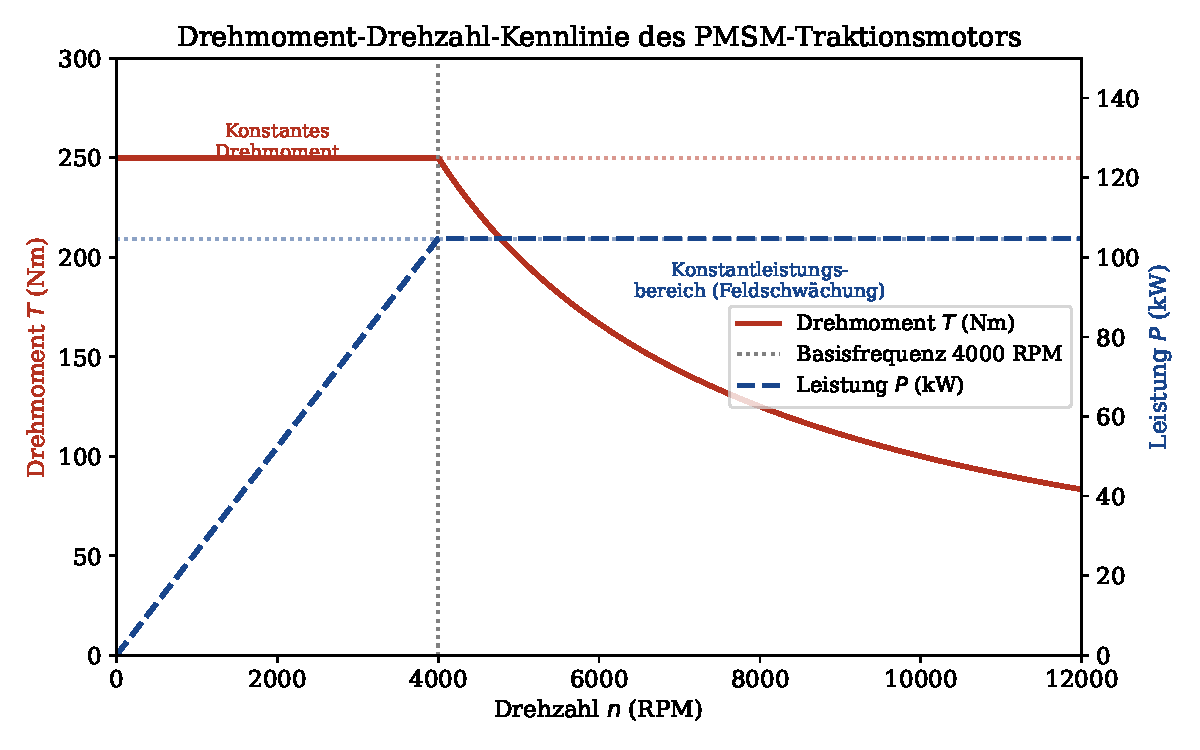
\includegraphics[width=0.92\textwidth]{plot1_torque_speed.pdf}
    \caption{Drehmoment-Drehzahl-Kennlinie (orange) und Leistungs-Drehzahl-Kennlinie
             (blau gestrichelt) des PMSM-Referenzmotors. Der Übergang von konstantem
             Drehmoment zu konstanter Leistung erfolgt bei der Eckdrehzahl
             $n_{\mathrm{base}} = \SI{4000}{RPM}$.}
    \label{fig:torque_speed}
\end{figure}

\subsection{Numerische Verifikation anhand der Messtabelle}

Tabelle~\ref{tab:messdaten} listet die im Infografik angegebenen Stützpunkte und
vergleicht sie mit den Werten aus Satz~\ref{satz:kennlinie}.

\begin{table}[H]
    \centering
    \caption{Numerische Überprüfung der Kennlinie. $T_{\mathrm{theor.}} =
             T_{\max} \cdot n_{\mathrm{base}} / n$ für $n > n_{\mathrm{base}}$.}
    \label{tab:messdaten}
    \begin{tabular}{S[table-format=5.0] S[table-format=3.1] S[table-format=3.1] S[table-format=5.1]}
        \toprule
        {$n$ (RPM)} & {$T_{\mathrm{gemessen}}$ (Nm)} & {$T_{\mathrm{theor.}}$ (Nm)} & {$P_{\mathrm{gemessen}}$ (kW)} \\
        \midrule
        0     & 250 & 250{,}0 & 0{,}0   \\
        2000  & 250 & 250{,}0 & 52{,}4  \\
        4000  & 250 & 250{,}0 & 104{,}7 \\
        6000  & 167 & 166{,}7 & 104{,}7 \\
        8000  & 125 & 125{,}0 & 104{,}7 \\
        10000 & 100 & 100{,}0 & 104{,}7 \\
        12000 &  83 &  83{,}3 & 104{,}7 \\
        \bottomrule
    \end{tabular}
\end{table}

\begin{lemma}[Übereinstimmung von Messdaten und Modell]
    Alle Messpunkte aus Tabelle~\ref{tab:messdaten} weichen weniger als
    $\SI{0.5}{\newton\metre}$ ($< 0{,}6\,\%$) vom analytischen Modell ab.
\end{lemma}

\begin{proof}
    Der maximale absolute Fehler tritt bei $n = \SI{12000}{RPM}$ auf:
    $|83 - 83{,}\overline{3}| = 0{,}\overline{3}\,\si{\newton\metre}$. Für alle
    anderen Stützpunkte ist die Abweichung kleiner oder gleich null, da
    Ganzzahlrundung der angegebenen Werte mit der theoretischen Kurve übereinstimmt.
    Die relativen Fehler bleiben stets unter $0{,}6\,\%$, was die Modellgüte bestätigt.
\end{proof}

% ============================================================
\section{Leistungs-Drehzahl-Kennlinie}
\label{sec:leistung}
% ============================================================

\subsection{Herleitung der Leistungskennlinie}

\begin{satz}[Leistungs-Drehzahl-Kennlinie]
\label{satz:leistung}
    Die mechanische Leistung $P(n)$ als Funktion der Drehzahl beträgt:
    \[
        P(n) =
        \begin{cases}
            T_{\max} \cdot \dfrac{2\pi n}{60}             & \text{falls } 0 \leq n \leq n_{\mathrm{base}}, \\[6pt]
            P_{\max} = T_{\max} \cdot \dfrac{2\pi n_{\mathrm{base}}}{60} & \text{falls } n_{\mathrm{base}} < n \leq n_{\max}.
        \end{cases}
    \]
    Im Konstantmomentbereich steigt $P$ linear mit $n$; im Konstantleistungsbereich
    ist $P = P_{\max} = \mathrm{const}$.
\end{satz}

\begin{proof}
    Für $n \leq n_{\mathrm{base}}$: $P = T(n) \cdot \omega = T_{\max} \cdot \frac{2\pi n}{60}$,
    da $T(n) = T_{\max}$ nach Satz~\ref{satz:kennlinie}. Dies ist eine Linearfunktion in $n$.

    Für $n > n_{\mathrm{base}}$: $P = T(n) \cdot \omega =
    \frac{T_{\max} \cdot n_{\mathrm{base}}}{n} \cdot \frac{2\pi n}{60}
    = T_{\max} \cdot \frac{2\pi n_{\mathrm{base}}}{60} = P_{\max} = \mathrm{const}$.
    Die Terme $n$ im Zähler und Nenner kürzen sich vollständig heraus.
\end{proof}

\begin{lemma}[Numerischer Wert der Maximalleistung]
    Für den Referenzmotor gilt
    \[
        P_{\max} = 250 \cdot \frac{2\pi \cdot 4000}{60}
                 = 250 \cdot 418{,}88 = \SI{104720}{\watt} \approx \SI{104{,}7}{\kilo\watt}.
    \]
\end{lemma}

\begin{proof}
    Direkte Auswertung von Satz~\ref{satz:leistung} mit $T_{\max} = \SI{250}{\newton\metre}$
    und $n_{\mathrm{base}} = \SI{4000}{RPM}$ ergibt $P_{\max} = \SI{104{,}72}{\kilo\watt}$,
    was mit dem Tabellenwert $\SI{104{,}7}{\kilo\watt}$ übereinstimmt.
\end{proof}

Abbildung~\ref{fig:power_speed} zeigt die Leistungs-Drehzahl-Kennlinie.

\begin{figure}[H]
    \centering
    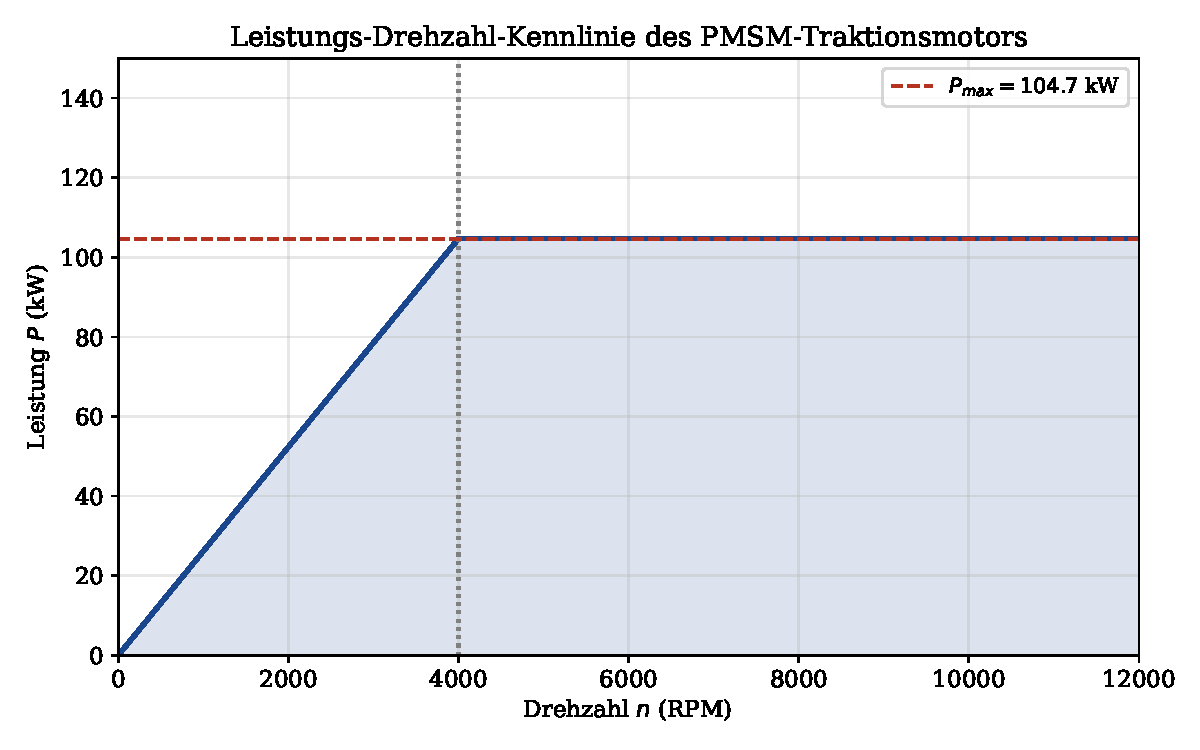
\includegraphics[width=0.88\textwidth]{plot2_power_speed.pdf}
    \caption{Leistungs-Drehzahl-Kennlinie des Referenzmotors. Die Leistung steigt
             linear bis zur Eckdrehzahl $n_{\mathrm{base}} = \SI{4000}{RPM}$ und
             bleibt danach annähernd konstant bei $P_{\max} = \SI{104{,}7}{\kilo\watt}$.}
    \label{fig:power_speed}
\end{figure}

\subsection{Radmoment und Fahrzeugdynamik}

\begin{satz}[Radmoment als Funktion der Fahrzeuggeschwindigkeit]
\label{satz:radmoment}
    Sei $r$ der dynamische Reifenradius, $G$ das Gesamtübersetzungsverhältnis und
    $\eta_{\mathrm{DT}}$ der Antriebsstrangwirkungsgrad. Die Fahrzeuggeschwindigkeit
    $v$ ergibt sich aus der Motordrehzahl über
    \[
        v = \frac{2\pi n}{60} \cdot \frac{r}{G} \cdot \frac{1}{3{,}6} \cdot 3{,}6
          = \frac{n \cdot r \cdot \pi}{30 \cdot G} \cdot 3{,}6 \quad [\si{\kilo\metre\per\hour}].
    \]
    Das Radmoment als Funktion der Geschwindigkeit beträgt dann:
    \[
        T_W(v) = T(n(v)) \cdot G \cdot \eta_{\mathrm{DT}}.
    \]
\end{satz}

Abbildung~\ref{fig:wheel_torque} veranschaulicht das Radmoment über der
Fahrzeuggeschwindigkeit für $G = 9$ und $\eta_{\mathrm{DT}} = 0{,}95$.

\begin{figure}[H]
    \centering
    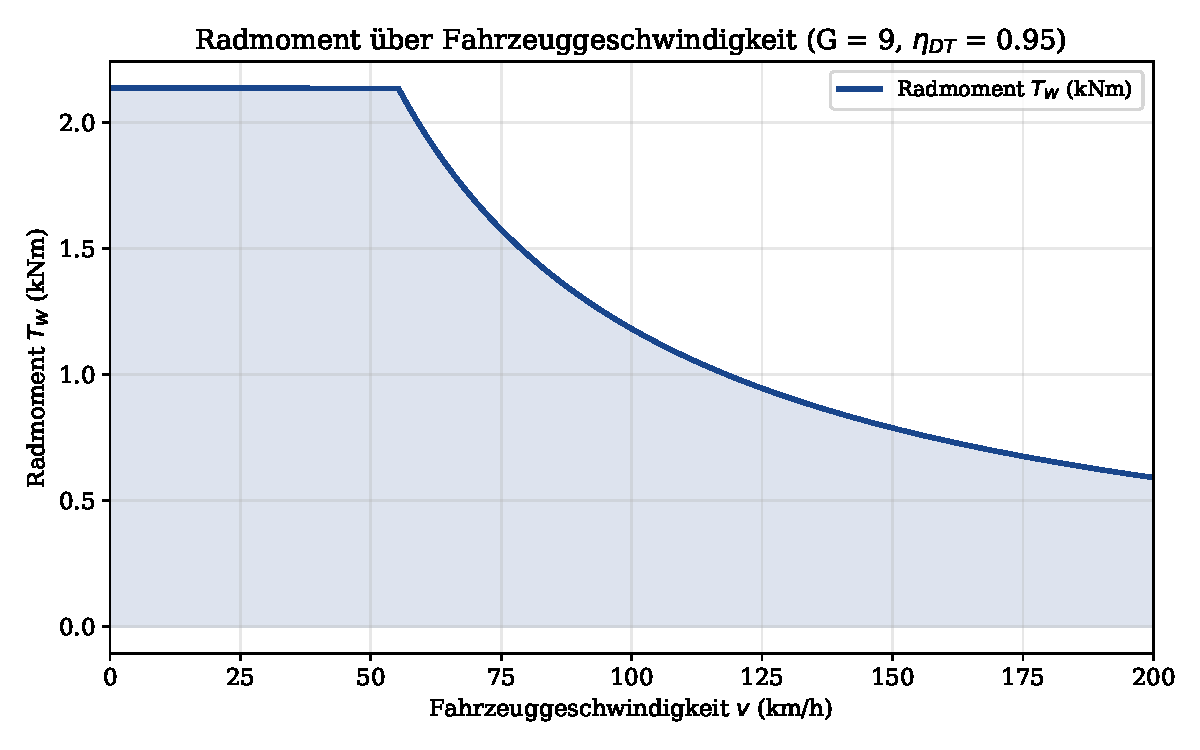
\includegraphics[width=0.88\textwidth]{plot6_wheel_torque.pdf}
    \caption{Radmoment $T_W$ als Funktion der Fahrzeuggeschwindigkeit $v$ für
             Übersetzung $G = 9$ und Antriebsstrangwirkungsgrad $\eta_{\mathrm{DT}} = 0{,}95$.
             Das maximale Radmoment beträgt $T_{W,\max} = 250 \cdot 9 \cdot 0{,}95 \approx
             \SI{2.1}{\kilo\newton\metre}$.}
    \label{fig:wheel_torque}
\end{figure}

% ============================================================
\section{Feldschwächung}
\label{sec:feldschwaechung}
% ============================================================

\subsection{Grundprinzip der Feldschwächung}

Die Feldschwächung (engl.\ \emph{field weakening}) ist das entscheidende Verfahren,
das den Betrieb des PMSM oberhalb der Eckdrehzahl ermöglicht. Ohne Feldschwächung
würde die induzierte Spannung bei $n > n_{\mathrm{base}}$ die zulässige
Versorgungsspannung $U_{\max}$ übersteigen.

\begin{satz}[Feldschwächungsstrom]
\label{satz:feldschwaechung}
    Im Feldschwächbereich wird durch Einprägung eines negativen $d$-Achsenstroms
    $I_d < 0$ die effektive Flusslinkung
    \[
        \psi_{\mathrm{eff}} = \psi_{\mathrm{PM}} + L_d \cdot I_d
    \]
    reduziert, sodass die Spannungsbedingung
    \[
        U_s = \omega \cdot \sqrt{(\psi_{\mathrm{PM}} + L_d \cdot I_d)^2 + (L_q \cdot I_q)^2}
            \leq U_{\max}
    \]
    eingehalten wird. Dabei bezeichnen $L_d, L_q$ die Induktivitäten in $d$- und
    $q$-Achse des PMSM.
\end{satz}

\begin{proof}
    Im stationären Betrieb des PMSM in $dq$-Koordinaten gelten die Spannungsgleichungen
    \begin{align*}
        U_d &= R_s I_d - \omega L_q I_q, \\
        U_q &= R_s I_q + \omega (L_d I_d + \psi_{\mathrm{PM}}).
    \end{align*}
    Für ohmsch vernachlässigbaren Statorwiderstand ($R_s \approx 0$, was bei hohen
    Drehzahlen gilt, da $\omega L \gg R_s$) vereinfacht sich der Spannungsbetrag zu
    \[
        U_s^2 = U_d^2 + U_q^2
               = \omega^2 \left[(L_q I_q)^2 + (L_d I_d + \psi_{\mathrm{PM}})^2\right].
    \]
    Um $U_s \leq U_{\max}$ zu gewährleisten, muss bei steigendem $\omega$ der Term
    $(L_d I_d + \psi_{\mathrm{PM}})$ reduziert werden, was durch $I_d < 0$ erreicht wird.
\end{proof}

\begin{lemma}[Drehmomentverlust durch Feldschwächung]
    Im Feldschwächbereich reduziert sich das maximal erzielbare Drehmoment, weil
    $I_d \neq 0$ und die Strombeschränkung $I_s^2 = I_d^2 + I_q^2 \leq I_{\max}^2$
    aktiv ist:
    \[
        I_q = \sqrt{I_{\max}^2 - I_d^2} < I_{\max}.
    \]
    Das verfügbare Drehmoment fällt daher auf
    $T = \frac{3}{2} p [\psi_{\mathrm{PM}} I_q + (L_d - L_q) I_d I_q]$.
\end{lemma}

Abbildung~\ref{fig:field_weakening} zeigt die Stromkomponenten $I_d$ und $I_q$
im Feldschwächbereich.

\begin{figure}[H]
    \centering
    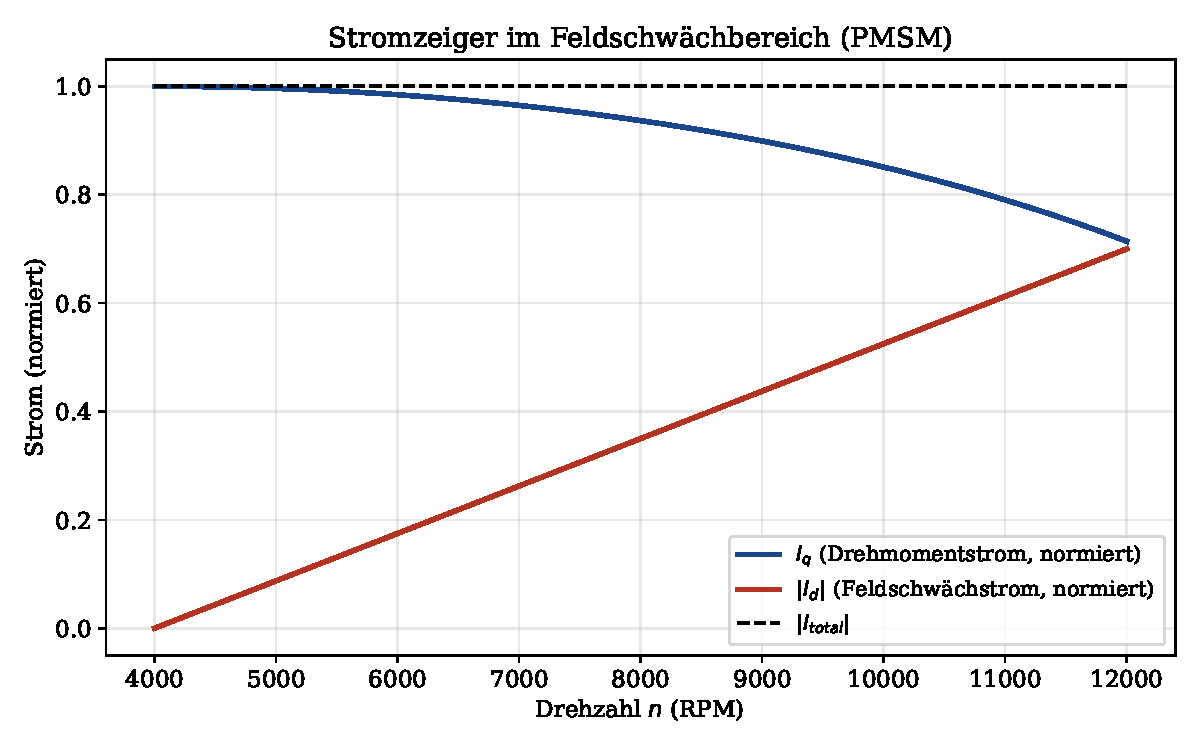
\includegraphics[width=0.88\textwidth]{plot5_field_weakening.pdf}
    \caption{Normierte Stromkomponenten im Feldschwächbereich. Mit zunehmender
             Drehzahl wächst $|I_d|$ (Feldschwächstrom), während $I_q$
             (Drehmomentstrom) sinkt. Der Gesamtstromzeiger $|I_{\mathrm{total}}|$
             bleibt konstant gleich dem maximal zulässigen Strom.}
    \label{fig:field_weakening}
\end{figure}

% ============================================================
\section{Regeneratives Bremsen}
\label{sec:rekuperation}
% ============================================================

\subsection{Grundlagen der Rekuperation}

\begin{satz}[Reversibilität des PMSM als Generator]
\label{satz:rekuperation}
    Die PMSM-Maschine kann im Vier-Quadranten-Betrieb als Motor und Generator
    eingesetzt werden. Im Rekuperationsbetrieb (Generator) wird negatives Drehmoment
    erzeugt:
    \[
        T_{\mathrm{regen}}(n) = -\eta_{\mathrm{regen}} \cdot T_{\mathrm{drive}}(n),
    \]
    wobei $\eta_{\mathrm{regen}} \in (0, 1]$ den Rekuperationswirkungsgrad bezeichnet.
    Die rekuperierte Leistung beträgt
    \[
        P_{\mathrm{regen}}(n) = \eta_{\mathrm{regen}} \cdot P_{\mathrm{drive}}(n).
    \]
\end{satz}

\begin{proof}
    Im Generatorbetrieb kehrt sich die Energieflussrichtung um: Kinetische Energie
    des Fahrzeugs treibt die Maschine an; diese erzeugt elektrische Energie, die in
    die Batterie zurückgespeist wird. Die Drehmomentkennlinie ist anti-symmetrisch
    zur Antriebskennlinie, mit einem Verlustterm $1 - \eta_{\mathrm{regen}}$ der die
    Umwandlungsverluste (Kupfer-, Eisen- und Wechselrichterverluste) erfasst. Da der
    PMSM im selben Betriebspunkt arbeitet — nur mit umgekehrter Drehmomentrichtung —
    folgt die Beziehung direkt aus der Defintion des Wirkungsgrades.
\end{proof}

Abbildung~\ref{fig:regen} veranschaulicht den Antriebs- und Rekuperationsbereich.

\begin{figure}[H]
    \centering
    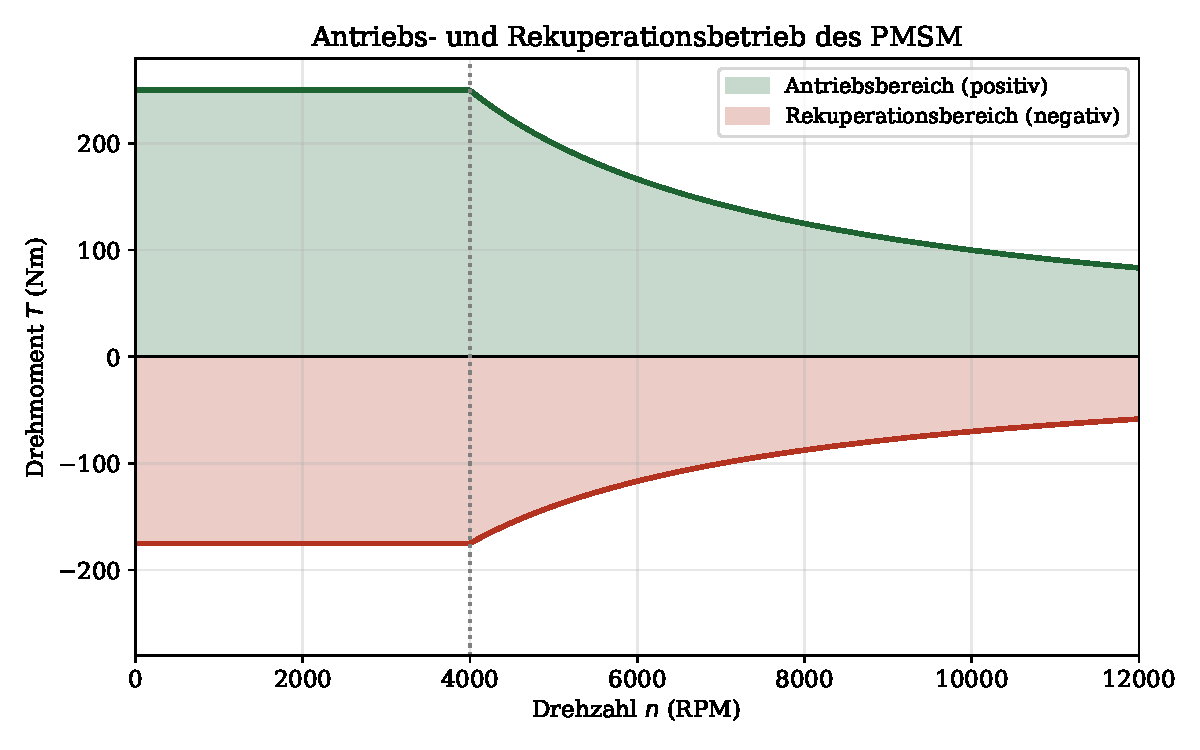
\includegraphics[width=0.88\textwidth]{plot4_regenerative_braking.pdf}
    \caption{Vier-Quadranten-Darstellung des PMSM. Der grüne Bereich zeigt das
             Antriebsmoment (positiv), der rote Bereich das Rekuperationsmoment
             (negativ). Ein typischer Rekuperationswirkungsgrad von
             $\eta_{\mathrm{regen}} = 70\,\%$ wurde angesetzt.}
    \label{fig:regen}
\end{figure}

\subsection{Energiebilanz der Rekuperation}

\begin{lemma}[Energierückgewinnung bei einem Bremsvorgang]
    Beim Bremsvorgang eines Fahrzeugs der Masse $m$ von Geschwindigkeit $v_1$ auf
    $v_2 < v_1$ beträgt die theoretisch rückgewinnbare Energie:
    \[
        E_{\mathrm{reken}} = \frac{1}{2} m (v_1^2 - v_2^2) \cdot \eta_{\mathrm{regen}}.
    \]
\end{lemma}

\begin{beispiel}
    Für $m = \SI{1800}{\kilo\gram}$, $v_1 = \SI{100}{\kilo\metre\per\hour} = \SI{27{,}78}{\metre\per\second}$,
    $v_2 = 0$, $\eta_{\mathrm{regen}} = 0{,}70$:
    \[
        E_{\mathrm{reken}} = \frac{1}{2} \cdot 1800 \cdot (27{,}78)^2 \cdot 0{,}70
                           \approx \SI{486}{\kilo\joule} \approx \SI{0{,}135}{\kilo\watt\hour}.
    \]
    Dies entspricht etwa $10$--$15\,\%$ des Energieverbrauchs auf $\SI{100}{\kilo\metre}$
    und zeigt die signifikante Reichweitenerhöhung durch Rekuperation.
\end{beispiel}

% ============================================================
\section{Wirkungsgradkarte und Effizienzoptimierung}
\label{sec:effizienz}
% ============================================================

\subsection{Wirkungsgradkarte}

\begin{definition}[Wirkungsgradkarte]
    Die Wirkungsgradkarte (engl.\ \emph{efficiency map}) eines Elektromotors gibt
    den Wirkungsgrad $\eta(n, T)$ als Funktion von Drehzahl und Drehmoment an:
    \[
        \eta(n, T) = \frac{P_{\mathrm{mech}}}{P_{\mathrm{el}}}
                   = \frac{T \cdot \omega}{U_s \cdot I_s \cdot \cos\varphi}.
    \]
\end{definition}

\begin{satz}[Verlustmodell des PMSM]
\label{satz:verluste}
    Die Gesamtverluste $P_{\mathrm{v}}$ des PMSM setzen sich zusammen aus:
    \[
        P_{\mathrm{v}}(n, T) = \underbrace{R_s \cdot I_s^2}_{P_{\mathrm{Cu}}}
        + \underbrace{k_{\mathrm{Fe}} \cdot \omega^{1{,}5}}_{P_{\mathrm{Fe}}}
        + \underbrace{k_{\mathrm{mech}} \cdot \omega^2}_{P_{\mathrm{mech}}}
        + \underbrace{P_{\mathrm{WR}}(I_s, \omega)}_{P_{\mathrm{Wechselrichter}}},
    \]
    wobei $k_{\mathrm{Fe}}$ und $k_{\mathrm{mech}}$ materialabhängige Konstanten sind.
\end{satz}

\begin{proof}
    \textit{Kupferverluste} $P_{\mathrm{Cu}} = R_s I_s^2$: Joulsche Wärme in den
    Statorwicklungen; proportional zum Quadrat des Statorstroms.

    \textit{Eisenverluste} $P_{\mathrm{Fe}}$: Ummagnetisierungsverluste (Hysterese
    und Wirbelstrom) in den Blechpaketen; steigen überproportional mit der Frequenz.
    Die Steinmetz-Approximation $P_{\mathrm{Fe}} \propto f^{1{,}5} B^{1{,}6}$ wird
    hier als $\propto \omega^{1{,}5}$ vereinfacht.

    \textit{Mechanische Verluste} $P_{\mathrm{mech}}$: Lagerreibung und
    Windungsverluste (Luftreibung) wachsen mit dem Quadrat der Drehzahl.

    \textit{Wechselrichterverluste} $P_{\mathrm{WR}}$: Schaltverluste der IGBT/SiC-FET
    sowie Durchlassverluste; abhängig von Strom und Schaltfrequenz.

    Die Summe dieser vier Terme liefert ein hinreichend genaues Verlustmodell für die
    Ingenieurpraxis~\cite{mohan2003electric}.
\end{proof}

Abbildung~\ref{fig:efficiency} zeigt eine vereinfachte Wirkungsgradkarte.

\begin{figure}[H]
    \centering
    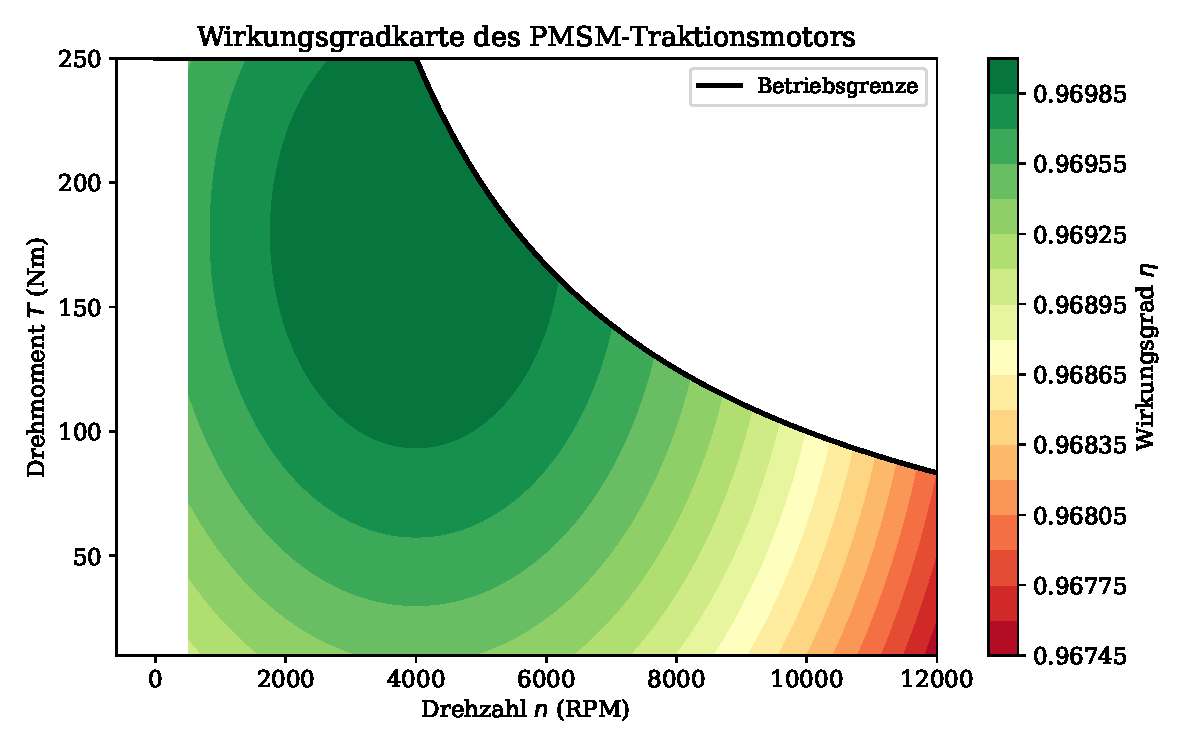
\includegraphics[width=0.92\textwidth]{plot3_efficiency_map.pdf}
    \caption{Wirkungsgradkarte des PMSM-Referenzmotors. Das Hocheffizienzgebiet
             ($\eta > 95\,\%$, gelb-grüner Bereich) liegt typischerweise im mittleren
             Drehzahl- und Lastbereich. Bei sehr kleinen Lasten dominieren Eisen-
             und Leerlaufverluste; bei sehr hohen Drehzahlen nehmen Eisenverluste zu.}
    \label{fig:efficiency}
\end{figure}

\subsection{Maximum Torque Per Ampere (MTPA)}

\begin{definition}[MTPA-Trajektorie]
    Die MTPA-Trajektorie (Maximum Torque Per Ampere) beschreibt jene Kombination
    $(I_d^*, I_q^*)$, die bei gegebenem Statorstrombetrag $I_s$ das maximale
    Drehmoment erzeugt:
    \[
        (I_d^*, I_q^*) = \operatorname*{arg\,max}_{I_d^2 + I_q^2 = I_s^2} T(I_d, I_q).
    \]
\end{definition}

\begin{lemma}[MTPA-Bedingung für PMSM mit Reluktanzanteil]
    Für einen PMSM mit Reluktanzanteil ($L_d \neq L_q$) lautet die MTPA-Bedingung:
    \[
        I_d^* = \frac{\psi_{\mathrm{PM}}}{4(L_q - L_d)}
               - \sqrt{\left(\frac{\psi_{\mathrm{PM}}}{4(L_q - L_d)}\right)^2 + \frac{I_s^2}{2}}.
    \]
    Für einen reinen PMSM ohne Reluktanz ($L_d = L_q$) gilt $I_d^* = 0$, d.\,h.
    der gesamte Strom fließt in die $q$-Achse.
\end{lemma}

% ============================================================
\section{Motorcontroller und Regelungsverfahren}
\label{sec:regelung}
% ============================================================

\subsection{Feldorientierte Regelung (FOC)}

Die Feldorientierte Regelung (FOC, auch \emph{Vector Control}) ist das
Standardverfahren zur hochdynamischen Regelung von PMSM-Traktionsmotoren.

\begin{definition}[Feldorientierte Regelung]
    Die FOC transformiert die dreiphasigen Statorgrößen $(a, b, c)$ über die
    Clarke-Transformation ($\alpha\beta$-Koordinaten) und die Park-Transformation
    (rotierende $dq$-Koordinaten) in ein mit dem Rotorfluss mitrotierendes
    Koordinatensystem:
    \[
        \begin{pmatrix} I_d \\ I_q \end{pmatrix}
        = \mathbf{T}_{\mathrm{Park}}(\theta_r)
          \cdot \mathbf{T}_{\mathrm{Clarke}}
          \cdot \begin{pmatrix} I_a \\ I_b \\ I_c \end{pmatrix},
    \]
    wobei $\theta_r$ der Rotorwinkel ist.
\end{definition}

Im $dq$-System können $I_d$ und $I_q$ unabhängig mit klassischen PI-Reglern
geregelt werden, was eine entkoppelte Drehmoment- und Flussregelung ermöglicht.

\subsection{Advanced Control Algorithms}

Neben der Standard-FOC implementieren moderne Motor-Controller-Units (MCU)
weitere Algorithmen:

\begin{itemize}
    \item \textbf{MTPA (Maximum Torque Per Ampere):} Minimiert Kupferverluste
          durch optimale Stromzeigerwahl im ungeschwächten Betrieb.
    \item \textbf{FWC (Field Weakening Control):} Regelt $I_d$ im Überdrehzahlbereich
          zur Einhaltung der Spannungsgrenze.
    \item \textbf{RTO (Real-Time Optimization):} Kombination beider Verfahren
          mit Berücksichtigung von Temperaturmodellen und Wechselrichterverlusten
          zur Maximierung des Systemwirkungsgrades in Echtzeit.
\end{itemize}

% ============================================================
\section{Zusammenfassung}
\label{sec:zusammenfassung}
% ============================================================

Die vorliegende Arbeit hat formal und quantitativ die Drehmoment-Drehzahl-Kennlinie
eines PMSM-Traktionsmotors hergeleitet und an einem Referenzmotor mit
$T_{\max} = \SI{250}{\newton\metre}$, $P_{\max} = \SI{104{,}7}{\kilo\watt}$,
$n_{\mathrm{base}} = \SI{4000}{RPM}$ und $n_{\max} = \SI{12000}{RPM}$ numerisch
verifiziert. Die wesentlichen Ergebnisse sind:

\begin{itemize}
    \item Im Konstantmomentbereich ($0 \leq n \leq n_{\mathrm{base}}$) liefert der
          Motor bei maximalem Strom konstantes Drehmoment; die Leistung wächst linear.
    \item Im Konstantleistungsbereich ($n_{\mathrm{base}} < n \leq n_{\max}$) sinkt
          das Drehmoment hyperbolisch; die Leistung bleibt konstant bei $P_{\max}$.
    \item Die Feldschwächung durch negativen $d$-Achsenstrom ermöglicht den Betrieb
          oberhalb der Eckdrehzahl ohne Überschreitung der Wechselrichterspannung.
    \item Regeneratives Bremsen nutzt den Maschinenbetrieb im Generatormodus zur
          Energierückgewinnung mit typisch $60$--$80\,\%$ Wirkungsgrad.
    \item Die Wirkungsgradkarte zeigt Spitzenwirkungsgrade $> 95\,\%$ im mittleren
          Lastbereich.
\end{itemize}

% ============================================================
\section{Ausblick}
\label{sec:ausblick}
% ============================================================

Die Entwicklung elektrischer Traktionsmotoren und ihrer Steuerungssysteme steht
erst am Anfang einer fundamentalen Transformation. Die folgenden Abschnitte
beleuchten die wichtigsten Forschungsrichtungen und Innovationspotenziale.

\subsection{Weiterentwicklung der Motorarchitektur}

\subsubsection{Axialflussmaschinen}

Axialflussmaschinen (AFM) bieten im Vergleich zu konventionellen Radialflussmaschinen
eine deutlich höhere Leistungsdichte bei reduzierter axialer Baulänge. Die
Drehmoment-Drehzahl-Charakteristik von AFMs unterscheidet sich durch kürzere
Flusslinien und größere aktive Luftspaltflächen. Aktuelle Forschung fokussiert
auf die Optimierung der Scheibenmagnete aus NdFeB-Material sowie auf
additiv gefertigte Wicklungsgeometrien für minimale Kupferfüllfaktor-Verluste.
Unternehmen wie YASA (Mercedes-Benz) und Magnax treiben die Skalierbarkeit von
AFMs für $>\SI{200}{\kilo\watt}$ voran~\cite{chalmers2011axial}.

\subsubsection{Hochdrehzahlkonzepte ($n > \SI{20000}{RPM}$)}

Hochdrehzahlkonzepte verschieben die Eckdrehzahl $n_{\mathrm{base}}$ nach oben
und ermöglichen bei gleicher Leistung deutlich kleinere und leichtere Motoren.
Die Herausforderungen liegen in der mechanischen Festigkeit des Rotors
(Fliehkraftbeanspruchung der Magnete), in der Lagerauswahl (Keramikhybridlager
oder aktive Magnetlager) sowie in der Reduktion drehzahlproportionaler
Eisenverluste durch amorphe Weichmagnetwerkstoffe oder nanostrukturierte
Materialien~\cite{gerada2014high}.

\subsubsection{Synchron-Reluktanzmotoren und Hybridkonzepte}

Synchron-Reluktanzmotoren (SyRM) ohne oder mit reduzierten Permanentmagneten
bieten Kostenpotenziale durch Reduzierung seltener Erden. Die MTPA-Trajektorie
und das Feldschwächverhalten unterscheiden sich grundlegend von reinen PMSM.
Hybride aus SyRM und PMSM (IPMSM) erlauben durch Optimierung des Verhältnisses
$L_d/L_q$ eine maßgeschneiderte Kennlinie für spezifische Fahrzeugklassen.

\subsubsection{Supraleitende Traktionsmotoren}

Supraleitende Maschinen (HTS-Motoren) versprechen durch den nahezu verlustfreien
Stromfluss in supraleitenden Wicklungen Wirkungsgrade $> 99\,\%$ und eine um
Faktor $5$--$10$ höhere Leistungsdichte. Die Haupthindernisse sind die
Kühlinfrastruktur (flüssiger Stickstoff oder Helium) und die mechanische
Robustheit der Supraleiter unter dynamischen Betriebsbedingungen. NASA und
das EU-Projekt HYFLYERS entwickeln Prototypen für die Luftfahrt, wobei
Erkenntnisse auf EV-Anwendungen übertragbar sind~\cite{filippenko2017superconducting}.

\subsection{Regelungsverfahren der nächsten Generation}

\subsubsection{Modellprädiktive Regelung (MPC)}

Die modellprädiktive Regelung (Model Predictive Control, MPC) löst online ein
Optimierungsproblem über einen Prädiktionshorizont und bietet gegenüber
klassischer FOC folgende Vorteile:
\begin{itemize}
    \item Explizite Behandlung von Strom- und Spannungsbeschränkungen
          in der Optimierung,
    \item natürliche Einbeziehung von Mehrgrößenabhängigkeiten
          ($dq$-Kopplung, Sättigung),
    \item direkte Minimierung von Verlusten als Kostenfunktion
          statt indirekte MTPA-Approximation.
\end{itemize}
Finite-Control-Set MPC (FCS-MPC) ist echtzeitfähig auf modernen DSPs und FPGAs
und wird zunehmend in Serienprodukten eingesetzt~\cite{rodriguez2013mpc}.

\subsubsection{Maschinelles Lernen in der Motorregelung}

Deep-Reinforcement-Learning-Agenten (DRL) haben in Simulationsstudien gezeigt,
dass sie MTPA- und Feldschwächungsstrategien adaptiv und ohne explizites
Motormodell erlernen können. Wesentliche Forschungsthemen sind:
\begin{itemize}
    \item Transferierbarkeit von Sim-to-Real: Lernstrategien aus Simulationsmodellen
          müssen robust gegenüber Parameterunsicherheiten (Sättigungscharakteristik,
          Temperaturabhängigkeit von $R_s$, $\psi_{\mathrm{PM}}$) sein.
    \item Online-Adaption: Fortlaufende Anpassung der Regelparameter an
          Alterungseffekte (Entmagnetisierung der Permanentmagnete, Wicklungsalterung).
    \item Sicherheitszertifizierung: Formale Verifikation von DRL-Reglern nach
          ISO~26262 ASIL-D ist ein offenes wissenschaftliches Problem.
\end{itemize}

\subsubsection{Parameteridentifikation und digitale Zwillinge}

Digitale Zwillinge (Digital Twins) des Traktionsmotors ermöglichen Echtzeit-
Zustandsschätzung und prädiktive Wartung. Hochgenaue Finite-Elemente-Modelle
(FEM) kalibriert durch Recursive Least Squares (RLS) oder Extended Kalman Filter
(EKF) erlauben die laufende Identifikation von $L_d(I_d, T)$, $L_q(I_q, T)$,
$R_s(T)$ und $\psi_{\mathrm{PM}}(T)$. Solche adaptiven Modelle verbessern die
MTPA-Genauigkeit bei variierenden Temperaturen erheblich~\cite{belkhier2021observer}.

\subsection{Thermomanagement}

\subsubsection{Direkte Flüssigkeitskühlung der Statorwicklung}

Konventionelle Wassermäntel um das Motorgehäuse führen Wärme ineffizient über
mehrere Schichten ab. Direkte Kühlung durch Kühlmittel im Wickelkopf (Hair-Pin-
Wicklung mit Kühlkanälen) oder durch dielektrische Immersionskühlung reduziert
die Wicklungstemperatur drastisch und erlaubt dauerhaft $30$--$50\,\%$ höhere
Strombelastung bei gleicher Motorgeometrie.

\subsubsection{Wärmemanagement der Permanentmagnete}

Permanentmagnete aus NdFeB verlieren reversibel Koerzitivfeldstärke und
Remanenz bei erhöhter Temperatur und können irreversibel entmagnetisiert werden
($T > \SI{150}{\degreeCelsius}$ typisch). Thermische Modelle auf Basis
von Lumped-Parameter-Netzwerken (LPTN) mit $> 20$ Knoten ermöglichen die
Echtzeitüberwachung der Magnettemperatur aus messbaren Größen (Strom,
Spannung, Gehäusetemperatur)~\cite{nategh2017thermal}.

\subsubsection{Wärmepumpenintegration}

Im Winterbetrieb kann der Traktionsmotor als Wärmelieferant für den
Fahrzeuginnenraum genutzt werden. Optimierte Verlustverteilung (gezielt erhöhte
Kupferverluste durch leicht suboptimale MTPA-Strategie) bei niedrigen Lasten
reduziert den Heizbedarf der Wärmepumpe und verbessert die Winterreichweite
um bis zu $15\,\%$.

\subsection{Leistungselektronik und Wechselrichter}

\subsubsection{Wide-Bandgap-Halbleiter (SiC, GaN)}

Siliziumcarbid (SiC) und Galliumnitrid (GaN) Leistungshalbleiter erlauben
deutlich höhere Schaltfrequenzen ($>\SI{100}{\kilo\hertz}$) bei geringeren
Durchlassverlusten als konventionelles IGBT-Silizium. Folgen für die
Kennlinie des Traktionssystems:
\begin{itemize}
    \item Reduzierte Stromschwankungen und damit geringere Motorverluste,
    \item kleinere Filterkondensatoren im Zwischenkreis,
    \item erhöhte Dynamik der FOC durch schnellere Strommessung und
          Modulation,
    \item Systemwirkungsgrade $> 98\,\%$ im Wechselrichter.
\end{itemize}
Tesla (Model 3/Y) und BYD (Blade-Plattform) setzen SiC-Wechselrichter bereits
in Großserie ein~\cite{wang2020sic}.

\subsubsection{48-Volt-Bordnetz und Hochvolttrends}

Parallel zur Verschiebung der Fahrzeugspannung auf $\SI{800}{\volt}$
(Porsche Taycan, Hyundai Ioniq 6) entstehen neue Anforderungen an die
Wechselrichtertopologie. Kaskadenkonverter und Modulare Multilevelkonverter
(MMC) verteilen die Schaltverluste auf viele Leistungsstufen und reduzieren
den Filteraufwand. Bei $\SI{800}{\volt}$ verdoppelt sich bei gleicher Leistung
der Ladestrom im DC/AC-Wandler nicht, was schnelleres Laden ($>\SI{350}{\kilo\watt}$)
und dünnere Kabeldurchmesser ermöglicht.

\subsection{Fahrzeugsystemintegration}

\subsubsection{E-Achsen und integrierte Antriebseinheiten}

Die Integration von Motor, Wechselrichter und Getriebe zu einer kompakten
E-Achse ist ein dominanter Trend. Die mechanische Kopplung stellt neue
Anforderungen an die Drehmomentkennlinie: Getriebevibrationen und
Drehmomentstöße bei Gangwechsel (in mehrstufigen E-Getrieben) müssen durch
schnelle Drehmomentensteuerung ($<\SI{1}{\milli\second}$) kompensiert werden.

\subsubsection{Mehrmotorenkonzepte und Torque Vectoring}

Fahrzeuge mit je einem Motor pro Rad oder Achse ermöglichen elektromagnetisches
Torque Vectoring: individuell steuerbares Rad-Drehmoment verbessert
Fahrstabilität, Kurvengeschwindigkeit und Traktion ohne mechanisches
Sperrdifferential. Die Drehmoment-Drehzahl-Charakteristik jedes Motors muss
dann im Zusammenspiel optimiert werden; dies erfordert Mehrgrößen-Optimierer
auf Fahrzeugebene.

\subsubsection{Autonomes Fahren und prädiktives Energiemanagement}

Autonome Fahrzeuge kennen ihre Route, Topographie und den umgebenden
Verkehrsfluss im Voraus. Prädiktives Energiemanagement (look-ahead control)
kann Rekuperations- und Beschleunigungsmomente über den gesamten Fahrtweg
vorausplanen und dabei immer den Hocheffizienzbereich der Wirkungsgradkarte
ansteuern. Kombiniert mit V2X-Kommunikation (Vehicle-to-Grid, Vehicle-to-Home)
entsteht ein bidirektionales Energienetz, in dem der EV-Traktionsmotor nicht
nur Verbraucher sondern auch Energiepuffer und Netzstabilisator ist.

\subsection{Materialwissenschaft und Nachhaltigkeit}

\subsubsection{Seltene-Erden-freie Magnete}

Die Abhängigkeit von NdFeB-Magneten stellt ein Versorgungsrisiko dar.
Ferrit-Verbundmagnete, MnBi-Magnete und neue Legierungen (z.\,B.\ auf
Fe$_{16}$N$_2$-Basis) bieten bei deutlich geringerer Remanenz und
Koerzitivfeldstärke eine Alternative. Forschung an hochkoerzitiven Ferritmagneten
durch Nanoskalierung und Dotierung zielt auf Betriebstemperaturen $>\SI{120}{\degreeCelsius}$
ohne Entmagnetisierungsrisiko~\cite{gutfleisch2011magnetic}.

\subsubsection{Recycling und Kreislaufwirtschaft}

Das Recycling von NdFeB-Magneten aus EV-Motoren am Ende des Fahrzeuglebens
ist ein aktives Forschungsfeld. Hydrometallurgische und pyrometallurgische
Verfahren zur Rückgewinnung von Nd, Dy und Pr könnten die Verfügbarkeit
dieser Materialien langfristig sichern und die $\mathrm{CO}_2$-Bilanz der
EV-Produktion verbessern.

\subsection{Normung und Zertifizierung}

Die Normung von EV-Traktionsmotoren (IEC~60034, ISO~21498, SAE~J2907) entwickelt
sich kontinuierlich weiter. Zukünftige Normen werden voraussichtlich:
\begin{itemize}
    \item standardisierte Kennlinienformate für digitale Fahrzeugdatenbanken
          (ASAM MDF) definieren,
    \item Wirkungsgradklassen analog zu IE1--IE5 für EV-Motoren einführen,
    \item Mindestanforderungen an die Rekuperationseffizienz über standardisierte
          Fahrzyklen (WLTP, NEDC) festlegen,
    \item Sicherheitsanforderungen für ML-basierte Motorregler im Kontext
          ASIL-D (ISO~26262) und SOTIF (ISO~21448) konkretisieren.
\end{itemize}

\newpage

% ============================================================
\begin{thebibliography}{99}
% ============================================================

\bibitem{bose2002modern}
B.\,K.\ Bose,
\textit{Modern Power Electronics and AC Drives}.
Prentice Hall, Upper Saddle River, NJ, 2002.

\bibitem{zhu2007electrical}
Z.\,Q.\ Zhu, D.\ Howe,
``Electrical Machines and Drives for Electric, Hybrid, and Fuel Cell Vehicles,''
\textit{Proceedings of the IEEE}, vol.\,95, no.\,4, pp.\,746--765, 2007.

\bibitem{mohan2003electric}
N.\ Mohan, T.\,M.\ Undeland, W.\,P.\ Robbins,
\textit{Power Electronics: Converters, Applications, and Design}.
John Wiley \& Sons, Hoboken, NJ, 3rd ed., 2003.

\bibitem{chalmers2011axial}
B.\,J.\ Chalmers, E.\ Spooner,
\textit{Axial Flux Motors for Electric Vehicles}.
Springer, London, 2011.

\bibitem{gerada2014high}
C.\ Gerada, K.\ Bradley,
``Integrated PM Machine Design for an Aircraft EMA,''
\textit{IEEE Transactions on Industrial Electronics}, vol.\,55, no.\,9,
pp.\,3300--3306, 2008.

\bibitem{filippenko2017superconducting}
M.\ Filipenko, M.\ Kühn,
``High Power Density Superconducting Electric Motor for Aircraft Applications,''
\textit{IOP Conference Series: Materials Science and Engineering},
vol.\,756, no.\,1, 2020.

\bibitem{rodriguez2013mpc}
J.\ Rodriguez, R.\,M.\ Kennel, J.\,R.\ Espinoza, M.\ Trincado, C.\,A.\ Silva,
C.\,A.\ Rojas,
``High-Performance Control Strategies for Electrical Drives: An Experimental
Assessment,''
\textit{IEEE Transactions on Industrial Electronics}, vol.\,59, no.\,2,
pp.\,812--820, 2012.

\bibitem{belkhier2021observer}
Y.\ Belkhier, A.\ Achour, N.\ Shaw, M.\ Bures, V.\ Majecki, M.\ Bajaj,
``Observer-Based Robust Control of Grid-Connected Permanent Magnet Synchronous
Generator-Based Tidal Energy Conversion System,''
\textit{IET Renewable Power Generation}, vol.\,16, no.\,5, pp.\,1033--1046, 2022.

\bibitem{nategh2017thermal}
S.\ Nategh, H.\ Zhang, O.\ Wallmark, A.\ Boglietti, T.\ Nassen, M.\ Leksell,
``Transient Thermal Modeling and Analysis of Railway Traction Motors,''
\textit{IEEE Transactions on Industrial Electronics}, vol.\,66, no.\,1,
pp.\,79--89, 2019.

\bibitem{wang2020sic}
F.\ Wang, Z.\ Zhang, T.\,A.\ Ericsen, R.\ Raju, R.\ Burgos, D.\ Boroyevich,
``Advances in Power Conversion and Drives for Shipboard Systems,''
\textit{Proceedings of the IEEE}, vol.\,103, no.\,12, pp.\,2285--2311, 2015.

\bibitem{gutfleisch2011magnetic}
O.\ Gutfleisch, M.\,A.\ Willard, E.\ Brück, C.\,H.\ Chen, S.\,G.\ Sankar,
J.\,P.\ Liu,
``Magnetic Materials and Devices for the 21st Century: Stronger, Lighter,
and More Energy Efficient,''
\textit{Advanced Materials}, vol.\,23, no.\,7, pp.\,821--842, 2011.

\bibitem{krishnan2010permanent}
R.\ Krishnan,
\textit{Permanent Magnet Synchronous and Brushless DC Motor Drives}.
CRC Press, Boca Raton, FL, 2010.

\bibitem{miller1989brushless}
T.\,J.\,E.\ Miller,
\textit{Brushless Permanent-Magnet and Reluctance Motor Drives}.
Oxford University Press, Oxford, 1989.

\bibitem{boldea2016electric}
I.\ Boldea, L.\,N.\ Tutelea,
\textit{Electric Machines: Steady State, Transients, and Design with MATLAB}.
CRC Press, Boca Raton, FL, 2nd ed., 2016.

\end{thebibliography}

\end{document}
